\chapter{Termo de Abertura do projeto}

\section{EAP}
\begin{figure}[!htb]
    \center{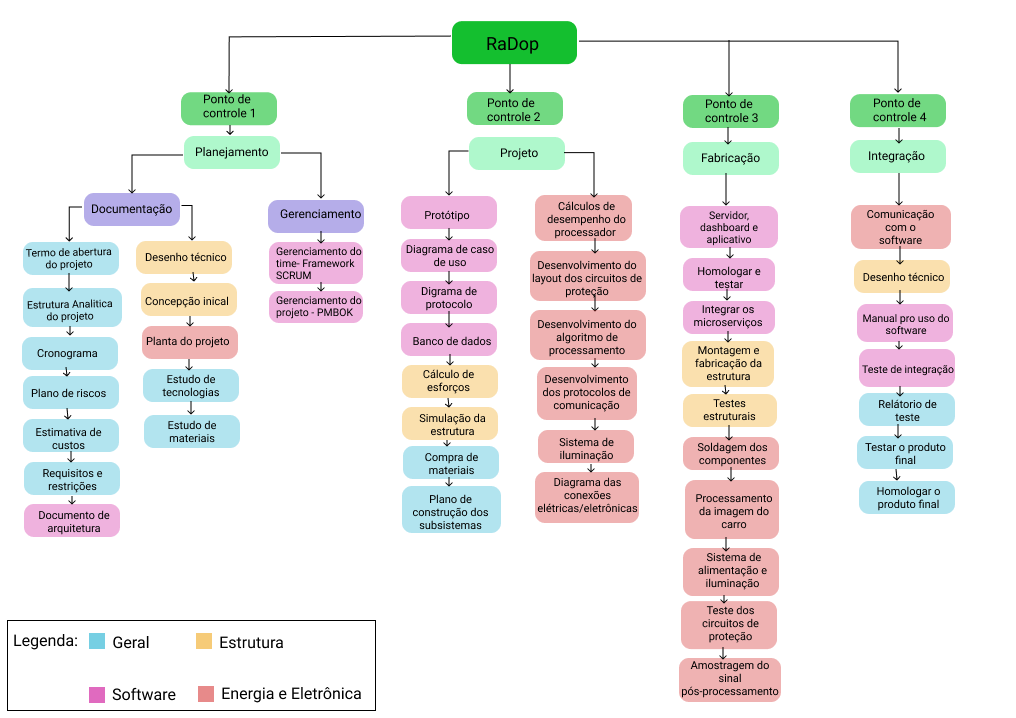
\includegraphics[width=\textwidth]{eap}}
    \caption{\label{fig:eap} EAP do projeto}
\end{figure}
\section{Lista É/Não é}
\subsection{É}
\subsection{Não é}
\section{Requisitos}
\subsection{Eletrônica}

Os requisitos de eletrônica são:
	
\begin{itemize}
	\item Detectar a aproximação do carro na via;
    \item Calcular a velocidade relativa do carro;
    \item Implementar uma comunicação entre os dois radares para determinar a emissão do alerta;
    \item Criar uma interface entre o radar e o motorista para visualização do alerta;
    \item Capturar imagem traseira do carro com a placa quando este passar acima da velocidade permitida;
    \item Projetar e construir circuitos de proteção para o dispositivos eletrônicos;
    \item Fazer o pré-processamento da imagem para reconhecimento da placa do veículo;
    \item Determinar a velocidade máxima do veículo para melhor captura da placa;
    \item Determinar a distância do veículo em relação ao radar para melhor captura da placa;
    \item Determinar a distância máxima entre os dois radares;
    \item Selecionar e implementar os protocolos de comunicação entre os dois radares;
    \item Selecionar e implementar os protocolos de comunicação entre os radares e o servidor;
     \item Determinar a capacidade de amarzenamento mínimo necessário para guardar dados quando a comunicação entre o radar e o servidor estiver fora de serviço;
     \item Determinar a velocidade mínima de transmissão de dados entre os radares para emissão de alerta;
     \item Determinar e implementar a estrutura do pacote de dados a ser enviado para o servidor contendo todas as informações necessárias;
     \item Transmitir para o servidor a velocidade, a imagem da placa pré-processada  e outras informações sobre o funcionamento do sistema.
\end{itemize}    
    
    As restrições de eletrônica são:

\begin{itemize}

	\item Se limitar em apenas reconhecer a placa do veículo, e não gerar a multa.
	\item Falha de comunicação entre os radares e o servidor por no máximo 3 dias.
	\item O veículo deve estar em uma velocidade igual ou menor que a velocidade máxima estabelecida para captura da placa.
	\item A captura da câmera deve ser apenas da traseira do veículo, devido a moto ter placa apenas na parte de trás, unificando o processo.
	\item A distância máxima entre os radares deve ser de 1 km.
	
\end{itemize} 	
	
\subsection{Energia}
\subsection{Estrutura}
\subsection{Software}

Os requisistos de software são:

\begin{itemize}
    \item Interface do Dashboard;
    \item Interface do Aplicativo;
    \item Manual de uso dos softwares (Microsserviços, Aplicativo e Dashboard);
    \item Funcionar com conexão a redes (Internet);
    \item Ser capaz de lidar e recuperar de falhas e erros (conexão, processamento e etc.);
    \item Softwares devem ser manuteníveis e evolutíveis;
    \item Softwares devem ser testáveis e testados;
    \item Software deve mostrar dados e informações do Radar;
    \item Software deve ser capaz de tomar decisões para alertar socorristas a respeito de prováveis acidentes automobilísticos;
    \item Software deve ser capaz de tomar decisões para alertar usuários de possíveis situações de risco;
    \item Software deve ser capaz de mostrar informações gerenciais com os dados do Radar;
\end{itemize}

As restrições de software são:

\begin{itemize}
    \item O software necessita estar sempre conectado à internet para comunicação e, consequentemente, para o correto funcionamento;
    \item O aplicativo de manutenção irá auxiliar apenas com o essencial;
    \item O aplicativo só funcionará em aparelhos Android;
    \item A linguagem de cada microsserviço (assim como framework/tecnologia) será definida dada necessidade (performance, armazemanento e etc) dos mesmos;
\end{itemize}

\section{\emph{Stakeholders}}
\section{Recurso humanos}
\section{Cronograma de atividades}
\section{Milestones Identificados}
\section{Estimativa de custos}

\subsection{Engenharia de Software}

Aqui está listado todos os gastos que serão necessários para a equipe de software, assim como todas as aquisições que serão feitas durante o projeto:

\begin{table}[]
    \resizebox{\textwidth}{!}{\begin{tabular}{@{}|c|c|c|c|c|c|c|@{}}
    \toprule
    \textbf{Nome do produto} & \textbf{Descrição}                      & \textbf{Marca} & \textbf{Preço unitário} & \textbf{Quantidade} & \textbf{Fornecedor} & \textbf{Orçamento} \\ \midrule
    Servidor                 & Máquina para execução dos serviços      & ---            & US\$ 10,00 por mês      & 5 meses             & Digital Ocean       & US\$ 50,00         \\ \midrule
    Raspberry Pi 3 B         & Placa de IoT para execução de softwares & Raspberry      & R\$ 279,90              & 1 unidade           & FilipeFlop          & R\$ 279,90         \\ \bottomrule
    \end{tabular}}
\end{table}

OBS: Essa planilha poderá ser atualizado dependendo de necessidades que surgirem durante a execução do projeto.

\section{Viabilidades financeira}
\section{Levantamento de riscos}
